\item \points{1b} {\bf Implement Step}

In the \texttt{protonet.py} file, complete the implementation of the \texttt{ProtoNet.\_step} method, which computes \eqref{eq:protonet_objective_minibatch} along with accuracy metrics. Pay attention to the inline comments and docstrings.
    
Assess your implementation on 5-way 5-shot Omniglot. To do so, run 
\begin{equation*} 
    \texttt{python protonet.py --num\_support 5} 
\end{equation*}

Use 15 query examples per class per task. Depending on how much memory your GPU has, you may want to adjust the batch size. Do not adjust the learning rate from its default of $0.001$.

To specify a non-default value for an argument, use the following syntax:
\begin{equation*}
    \texttt{python protonet.py --argument1 value1 --argument2 value2}
\end{equation*}

    As the model trains, model checkpoints and TensorBoard logs are periodically saved to a \texttt{log\_dir}. The default \texttt{log\_dir} is formatted from the arguments, but this can be overriden. You can visualize logged metrics by running
\begin{equation*}
    \texttt{tensorboard --logdir logs/}
\end{equation*}
and navigating to the displayed URL in a browser. If you are running on a remote computer with server capabilities, use the \texttt{--bind\_all} option to expose the web app to the network. Alternatively, consult the Azure guide for an example of how to tunnel/port-forward via SSH.

To resume training a model starting from a checkpoint at \texttt{\{some\_dir\}/state\{some\_step\}.pt}, run
\begin{equation*}
    \texttt{python protonet.py --log\_dir some\_dir --checkpoint\_step some\_step}
\end{equation*}

Your plot of the validation query accuracy over the course of training should look like the figure below.
\begin{center}
    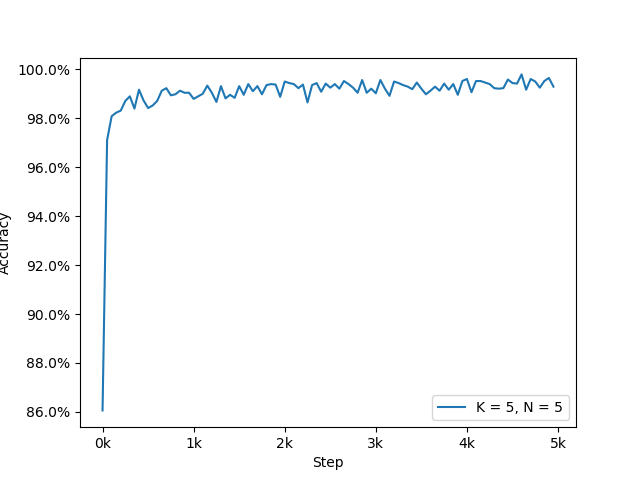
\includegraphics[width=0.75\linewidth]{./figures/protonets_q2}
\end{center}

\textbf{Hint}: you should obtain a query accuracy on the validation split of at least $99\%$.